\documentclass[
	a4paper, % Paper size, use either a4paper or letterpaper
	10pt, % Default font size, can also use 11pt or 12pt, although this is not recommended
	unnumberedsections, % Comment to enable section numbering
	twoside, % Two side traditional mode where headers and footers change between odd and even pages, comment this option to make them fixed
]{LTJournalArticle}

\addbibresource{sample.bib} % BibLaTeX bibliography file

% A shortened article title to appear in the running head, leave this command empty for no running head

% \footertext{\textit{Journal of Biological Sampling} (2024) 12:533-684} % Text to appear in the footer, leave this command empty for no footer text

\setcounter{page}{1} % The page number of the first page, set this to a higher number if the article is to be part of an issue or larger work

%----------------------------------------------------------------------------------------
%	TITLE SECTION
%----------------------------------------------------------------------------------------

\title{Design Exercise 2\\ Engineering Notebook} % Article title, use manual lines breaks (\\) to beautify the layout

% Authors are listed in a comma-separated list with superscript numbers indicating affiliations
% \thanks{} is used for any text that should be placed in a footnote on the first page, such as the corresponding author's email, journal acceptance dates, a copyright/license notice, keywords, etc
\author{%
	Adarsh Hiremath and Andrew Palacci
}


%----------------------------------------------------------------------------------------

\begin{document}

\maketitle % Output the title section

%----------------------------------------------------------------------------------------
%	ARTICLE CONTENTS
%----------------------------------------------------------------------------------------

\section{I. Introduction}
In our design exercise, we implemented a model of a small, asynchronous distributed system. In this system, each of the three simulated machines run at different clock rates assigned randomly at initialization. Each machine listens on a socket for incoming messages from other machines and updates the corresponding logical clock and message queue for each machine. In this engineering notebook, we intend to describe our design decisions and the results from the following experiments:
\begin{itemize}
    \item Five iterations of the scale model for exactly one minute. 
    \item A single run of the scale model for two minutes.
    \item Modifying the the probabilities that machines send messages to other machines. 
\end{itemize}

The source code for our chat application can be found \href{https://github.com/andrewp2303/logical_clocks}{here}.

\section{II. Model Distributed System Design}

Building our scale model for the simulated machines required implementing a protocol for the three machines to communicate. Otherwise, it would be impossible to receive logical clock information, send messages, or update the message queue. Thus, the first question Andrew and I sought to answer in the design process was what protocol we wanted to implement for our scale model. 

Initially, Andrew and I were inclined to implement our communication protocol using a simple peer-to-peer (P2P) networking library such as \href{https://pypi.org/project/pyp2p/}{Python's P2P}. The idea of P2P networking was appealing since there would be no single point of failure;  each machine could act as both a client and server, allowing for a more dynamic and flexible system. Additionally, with P2P, we thought that we could cut the number of connections in half because every connection would be bidirectional. 

However, we decided to use web sockets instead for a couple of reasons: 
\begin{itemize}
    \item By using web sockets, we could partially reuse implementations from the first design project instead of learning P2P networking for the first time for this project. 
    \item The problem specification recommended that each machine in the simulation send and receive information using web sockets. 
    \item Completely decentralizing communication is not realistic, especially at scale. It is far easier to accomodate more machines in a distributed system without dramatically revamping the code base when machines can ping a server without anything other than an endpoint. 
\end{itemize}

Instead of using a P2P system, we decided to implement a server and a client on each machine. In our code, the server exclusively listens for messages from other machines and the client sends messages to other machines in the model. Since we implemented the previous design project in Python, we did the same for this design project as well. 

\section{III. Five Scale Model Iterations}

We ran five simulations of our model distributed system, each for approximately a minute. During each simulation, we logged the message queue size and logical clock time for each machine after every completed tick of the machine. 
    
Initially, we logged the message queue size and logical clock time using Python's time module. However, unreliability in the time module and differences across machines prompted us to utilize the tick times from the simulations themselves. We initialized a variable, \texttt{currTime}, to 0 at the start of every thread. Then, at every operation, we incremented \texttt{currTime} until it hit the randomly generated \texttt{tickSize} for each machine. Then, we set \texttt{currTime} to 0 once again, repeating the process. Since each machine runs at a clock rate of 0 to 6 ticks per second, we were effectively able to simulate one "real" second on each simulated machine to log any necessary values for producing our graphs. 

We generated the following graphs for each trial: 

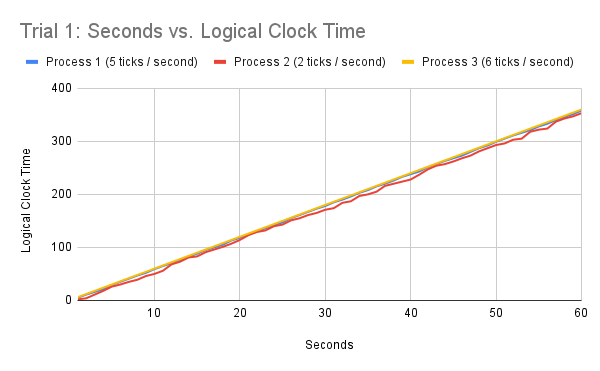
\includegraphics[width=7.8cm]{assets/t1_clock.png}
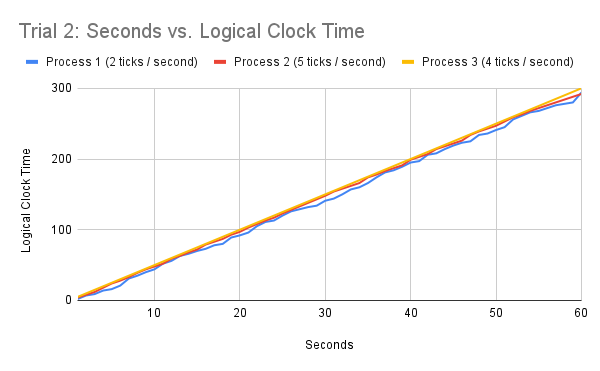
\includegraphics[width=7.8cm]{assets/t2_clock.png}
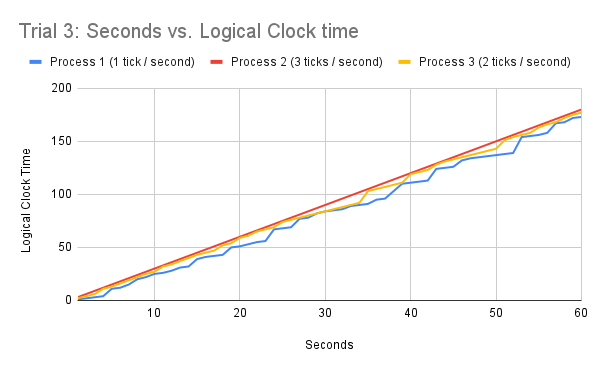
\includegraphics[width=7.8cm]{assets/t3_clock.png}
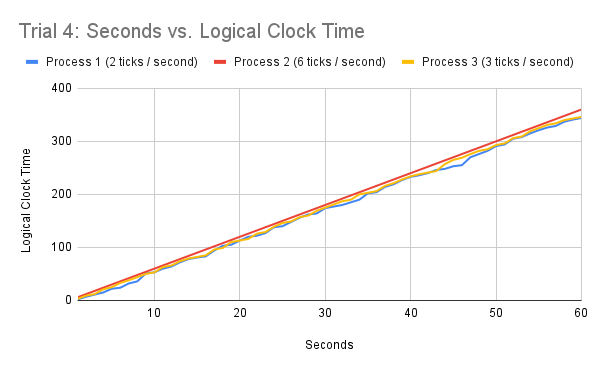
\includegraphics[width=7.8cm]{assets/t4_clock.png}
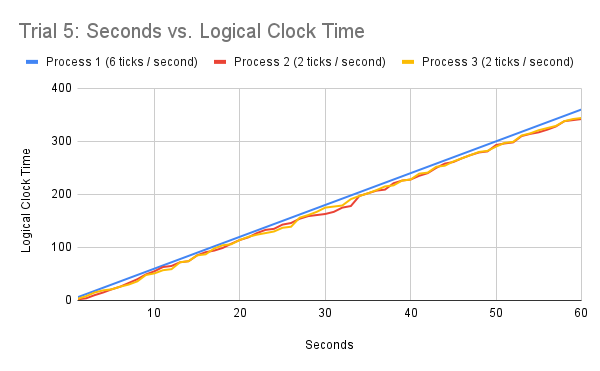
\includegraphics[width=7.8cm]{assets/t5_clock.png}
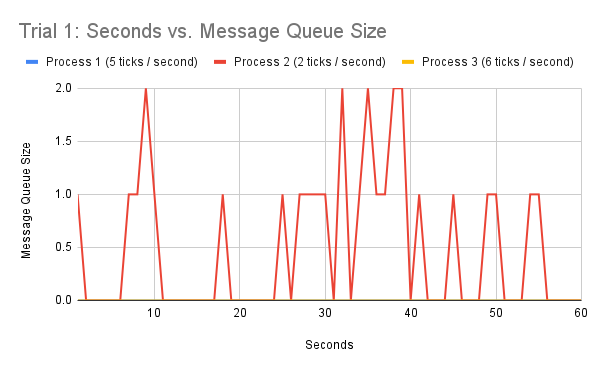
\includegraphics[width=7.8cm]{assets/t1_size.png}
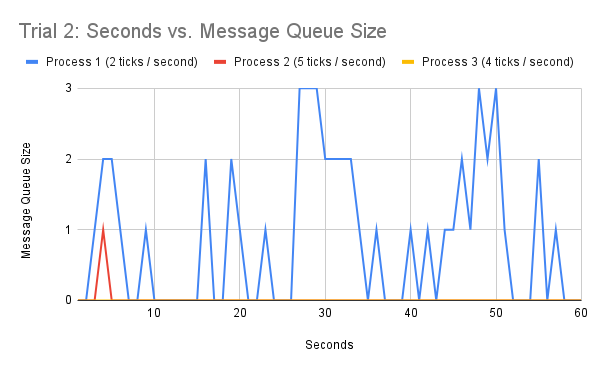
\includegraphics[width=7.8cm]{assets/t2_size.png}
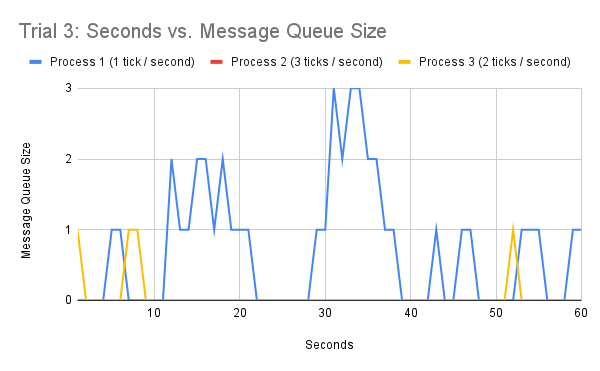
\includegraphics[width=7.8cm]{assets/t3_size.png}
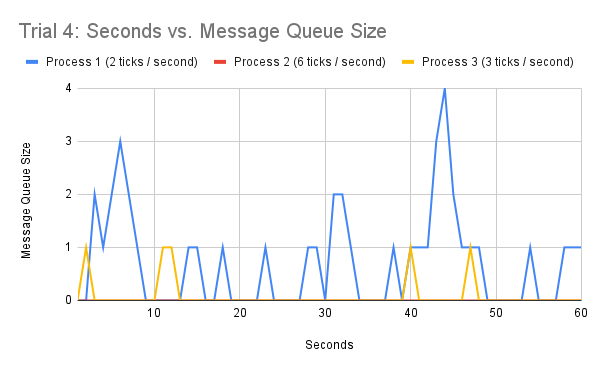
\includegraphics[width=7.8cm]{assets/t4_size.png}
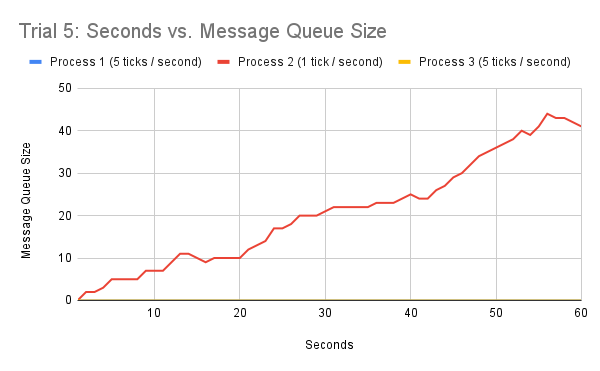
\includegraphics[width=7.8cm]{assets/t5_size.png}

\vspace{1mm}

After experimenting with our scale models and analyzing the above graphs, we noticed the following important trends: 
\begin{itemize}
    \item Processes runnning with less ticks per second had much larger jumps in logical clock time. This is best illustrated on the graph for trial 3 where process 1 ran at 1 tick / second, process 2 ran at 3 ticks / second, and process 3 ran at 2 ticks / second. The line for process 1 is the most jagged, demonstrating larger deviations  from the line of best fit. The line for process 3 is the second most jagged, with the line for process 2 following after. The jaggedness in these lines exponentially reduces, demonstrating that faster tick speeds also reduce variations in logical clock time. 
    \item Processes running with less ticks per second also struggled to manage the message queue size. This is illustrated well in the message queue graph for trial 1, where every process except the one running at 2 ticks / second had a queue length of 0 for the entirety of the simulation. This is logical because systems operating at a slower clock speed struggle to process inbound messages of peers running at comparatively higher clock speed (that thus send more messages).
\end{itemize}





% \section{IV. Longer Scale Model Iterations}

% \section{V. Modified Probabilities}

% \section{VI. Unit Testing}



\end{document}
